\subsection{A .net rendszer részei: GC, CIL, assembly-k. Esemény vezérelt programok felépítése windows alatt.}

\textbf{Problémák a natív nyelvben:}
\begin{itemize}
    \item \texttt{void*} típusú pointer, a memóriában lehet garázdálkodni vele
    \item inicializálatlan változó
    \item pointer, ami elkóborol
    \item kicímzés tömbből
    \item változók típusának máshogy értelmezése
    \item dinamikus változók törlésekor a memória fragmentálódik
    \item megoldás: néhány problémára a C++, a többire: menedzselt kód
    \item a menedzselt kód tartalmaz Garbage Collectort és indexhatár ellenőrzőt is
\end{itemize}

\textbf{GC -- Garbage Collector:}
\begin{itemize}
    \item automatikus szemétgyűjtés
    \item a már nem használt példányokat kitörli, memóriaterületet felszabadítja
    \item defragmentálja a memóriát
\end{itemize}

\begin{center}
    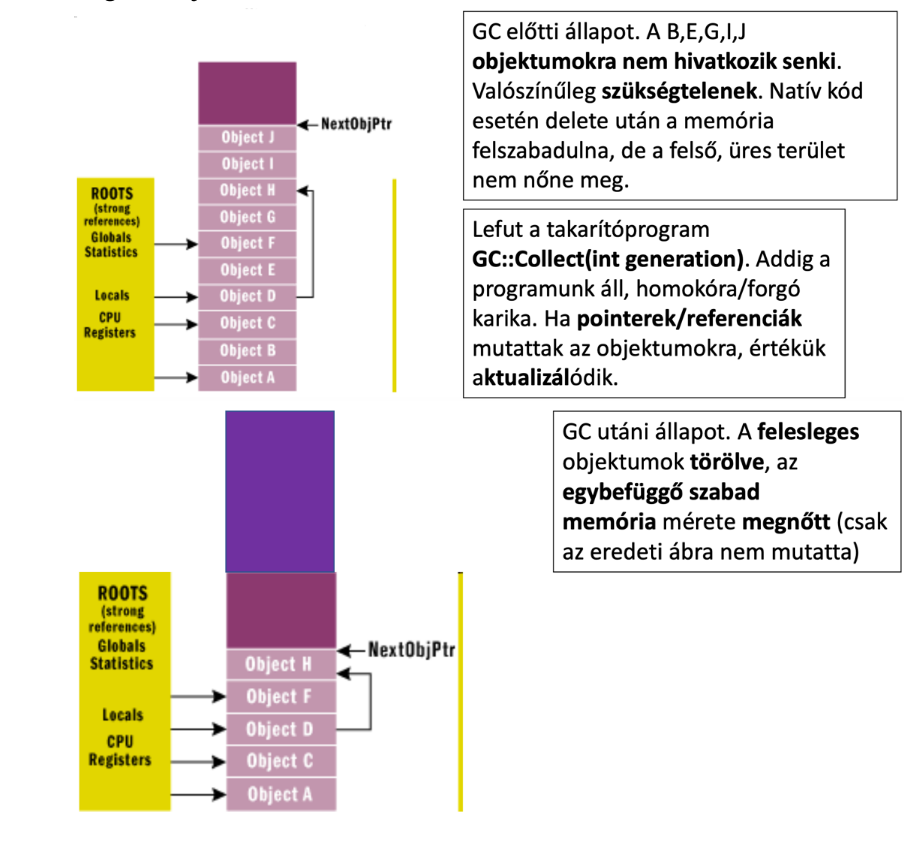
\includegraphics[width=0.9\textwidth]{res/imgs/info_19_gc.png}
\end{center}

\begin{itemize}
    \item memóriakezelő műveletek összehasonlítása:
\end{itemize}

\begin{table}[H]
    \centering
    \renewcommand{\arraystretch}{1.3}
    \begin{tabular}{|p{2cm}|p{2cm}|p{3.5cm}|p{3.5cm}|p{2cm}|}
        \hline
        \textbf{Alap C} & \textbf{C++} & \textbf{Managed C++} & \textbf{C++/CLI} & \textbf{C++/Cx} \\ \hline
        \texttt{malloc()} & \texttt{new} & \texttt{\_\_gc new} & \texttt{gcnew} & \texttt{ref new} \\ \hline
        \texttt{free()} & \texttt{delete: \~{}} & \texttt{nullptr, \~{}, !} & \texttt{nullptr, \~{}, !} & Mint a cli \\ \hline
        \texttt{Pointer(*)} & \texttt{Pointer(*)} & \texttt{\_\_nogc pointer(*)}, \newline \texttt{\_\_gc pointer(*)} & \texttt{Pointer(*)} natív terület, \newline \texttt{Handle(\^{})} GC halom & \\ \hline
    \end{tabular}
\end{table}

\textbf{CIL:}
\begin{itemize}
    \item common intermediate language
    \item a .NET nyelvek erre fordulnak le
    \item egy solution-ön belül lehet több nyelven programozni
    \item lehet menedzselt és natív kód egymás mellett
\end{itemize}

\textbf{.net keretrendszer:}
\begin{itemize}
    \item memóriakezelés: GC
    \item windows elemek típusai: assembly, Base Class Library-ben
    \item nyelvek: Visual Basic, C\#, C++/CLI
    \item CIL
    \item hálózat, periféria, adatbázis stb. elérés egyszerűsítve
\end{itemize}

\textbf{Assembly-k:}
\begin{itemize}
    \item RAD (gyors alkalmazásfejlesztés)
    \item ,,gyors'' -- előre elkészített elemek felhasználása
    \item assembly-k: gyártószerszámok
    \item statikus paraméterek: properties
    \item windows eseményre adott válasz: events
\end{itemize}

\textbf{Gyakran használt alapvezérlők:}
\begin{itemize}
    \item Form:
    \begin{itemize}
        \item nem rakható fel a toolbox-ból, új projektnél jön létre
        \item properties-ben találhatóak a beállításai
        \item programból: \texttt{this->Text}, mert a form egy referencia osztály
        \item eseménykezelő függvények megírása: villámra kattintva esemény kiválasztása, majd duplakatt
        \item üres helyre kettőt kattintva megnyílik az editor ablak
        \item alapméretezett esemény: \texttt{Load}
        \begin{itemize}
            \item erre az eseményre tesszük a programunk inicializáló részét
        \end{itemize}
        \item többi esemény: \texttt{Mouseclick}, \texttt{MouseDowns}, \texttt{MouseUp}, \texttt{MouseMove}, \texttt{KeyPress}, \texttt{KeyDown}, \texttt{KeyUp}, \texttt{Resize}, \texttt{Paint}, \texttt{FormClosing} (\texttt{e->Cancel=true}-val megakadályozható)
    \end{itemize}
    \item Label:
    \begin{itemize}
        \item szöveg kiírására
        \item \texttt{Text} property tartalmazza a szöveget
    \end{itemize}
    \item TextBox:
    \begin{itemize}
        \item szöveg bevitele
        \item esemény: \texttt{TextChanged}
    \end{itemize}
    \item Button:
    \begin{itemize}
        \item \texttt{Text} property
        \item \texttt{Click} esemény
    \end{itemize}
    \item checkBox:
    \begin{itemize}
        \item kijelölőnégyzet
    \end{itemize}
    \item RadioButton:
    \begin{itemize}
        \item kb. checkBox, de egy konténerobjektumon belül egyszerre egy lehet aktív
    \end{itemize}
    \item GroupBox
    \item HScrollBar, VScrollBar:
    \begin{itemize}
        \item csúszkák
    \end{itemize}
    \item NumericUpDown
    \item ComboBox, ListBox
    \item ProgressBar
\end{itemize}

\textbf{Ritkábban használt vezérlők:}
\begin{itemize}
    \item PictureBox
    \item Menük
    \item MenuStrip
    \item ContextMenuStrip
    \item ToolStrip
    \item StatusStrip
\end{itemize}

\textbf{Nem látható vezérlők:}
\begin{itemize}
    \item dialógusablakok: \texttt{OpenFileDialog}, \texttt{SaveFileDialog}, \texttt{PrintPreviewDialog}
    \item Timer
    \item SerialPort
\end{itemize}

\textbf{Eseményvezérelt programok felépítése:}
\begin{enumerate}
    \item program indul (kezdeti inicializálás)
    \item program végtelen ciklusban várakozik
    \item az operációs rendszerben történik valami (esemény)
    \item A program erre az eseményre reagál valamely programrészlet (függvény, vagy metódus) végrehajtásával. Ha voltak a felületen bemenő adatok, azokat beolvassa, eredményeket számít, majd megjelenít a felületen.
    \item várakozik (2. lépés) vagy amíg a ,,lépj ki'' esemény meg nem érkezik
    \item kilép
\end{enumerate}